%% ASI 2026 — Track II submission, IEEE conference style.
%% Template: IEEEtran (062824).
\documentclass[conference,10pt]{IEEEtran}
\IEEEoverridecommandlockouts

\usepackage{cite}
\usepackage{amsmath,amssymb,amsfonts}
\usepackage{graphicx}
\usepackage{booktabs}
\usepackage{xcolor}
\usepackage[inline]{enumitem}
\usepackage{etoolbox}
\usepackage{hyperref}
\hypersetup{
  colorlinks = true,
  linkcolor  = {blue!50!black},
  citecolor  = {blue!50!black},
  urlcolor   = {blue!50!black},
}

% --- Resilient \input ------------------------------------------------
% If a per-phase LaTeX table hasn't been generated yet, emit a clearly-
% marked placeholder rather than fail the build.
\newcommand{\inputiffile}[2]{%
  \IfFileExists{#1}{\input{#1}}{%
    \begin{table}[!ht]\centering\small
    \fbox{\parbox{0.9\linewidth}{\centering\itshape
      Placeholder for \texttt{\detokenize{#1}} --- run the corresponding
      phase to generate this table (#2).}}
    \end{table}}}

\title{Pathway-Informed Deep Learning for Multi-Phenotype Therapy-Response Stratification in TCGA-BRCA}

\author{%
\IEEEauthorblockN{Sujoy Banik, Koushik Howlader, Ushashi Bhattacharjee, Zainab Ghafoor,\\
Sayantan Chakraborty, Adrito Roy, Tanusree Bhattacharjee, Tirtho Roy}
\IEEEauthorblockA{\textit{TherapAgent Research Group}\\
Code and reproducible artifacts: \url{https://github.com/sujoy166/TherapAgent}}
}

\begin{document}
\maketitle

\begin{abstract}
Predicting whether a breast-cancer patient will receive targeted molecular
therapy, radiation therapy, and survive at least six months is intrinsically
a multi-label clinical decision driven by the joint activity of dozens of
biological pathways --- many of them immunological. We benchmark three
recently proposed pathway-informed neural architectures on a common substrate:
the Reactome-hierarchical BINN, the multi-head graph-attention GraphPath, and
the edge-aware Graph Transformer PATH. All three are applied to identical
data: ssGSEA scores over 1,686 Reactome pathways on 618 TCGA-BRCA samples,
predicting three independent binary phenotypes (TMT, RT, OS\,$\geq$\,180\,d).
We adapt each architecture to pathway-level inputs, replace the gene-level
CNV/mutation stages of GraphPath and PATH with a learnable per-pathway
projection, and apply a class-weighted BCE loss across all three heads.
Every phase of the pipeline (Reactome ingest, data preparation, training,
evaluation) emits a versioned LaTeX booktabs table; the publication figures
use the Okabe--Ito palette and viridis colormap for color-vision-deficiency
accessibility. On the held-out test set, PATH delivers the strongest TMT
discrimination (AUROC 0.642), BINN leads on OS (AUROC 0.650), and the three
models converge on the balanced RT head. Reactome's Immune System subtree
dominates the attended pathways across models, framing the result for the
ASI 2026 systems-immunology audience.
\end{abstract}

\begin{IEEEkeywords}
biologically informed neural networks, graph attention, graph transformer,
Reactome, ssGSEA, breast cancer, therapy-response prediction, multi-label
classification, systems immunology, interpretable deep learning.
\end{IEEEkeywords}

\section{Introduction}
Breast-cancer treatment is rarely a single decision: clinicians choose
whether to deliver targeted molecular therapy (TMT), whether to add radiation
(RT), and how those choices interact with the expected survival window. These
decisions are correlated but not redundant. A model that collapses them into
a single 8-class label discards the underlying biology; a model that treats
them independently can predict any combination, including rare ones, and
surfaces \emph{which} biological programmes drive \emph{which} decision.

Pathway-level activity, derived from gene-expression data via single-sample
gene-set enrichment analysis (ssGSEA~\cite{barbie2009ssgsea,subramanian2005gsea})
against the Reactome database~\cite{gillespie2022reactome}, gives a compact
and biologically interpretable input representation. Reactome's
\emph{Immune System} subtree alone covers hundreds of nodes spanning innate,
adaptive, cytokine, antigen-processing, and TCR/BCR signalling cascades, so a
sufficiently structured network can be read as a model-derived immune
programme for each therapy axis.

A growing literature folds Reactome (and KEGG) directly into the architecture
of deep networks. Three recent representatives anchor the design space:
\textbf{BINN}~\cite{hartman2023binn} (a sparse multi-layer perceptron whose
masks encode the Reactome parent-child hierarchy, generalising
P-NET~\cite{elmarakeby2021pnet} across modalities);
\textbf{GraphPath}~\cite{ma2024graphpath} (a multi-head graph attention
network~\cite{velickovic2018gat} over a pathway-pathway interaction graph);
and \textbf{PATH}~\cite{howlader2026path} (an edge-aware graph transformer
with Laplacian positional encoding, soft structural masking, edge-conditioned
attention bias, and FiLM~\cite{perez2018film}-modulated gene embeddings).
These three architectures span the natural design axis from sparse hierarchy
through graph attention to edge-aware transformer, yet have never been
compared on a common data flow: published evaluations differ in cancer type,
in label cardinality, in input modality, and in pathway database.

\paragraph*{Contributions.}
\begin{itemize}[leftmargin=*]
\item A common \emph{multi-label} benchmark on 618 TCGA-BRCA samples that
  bit-decodes a clinically meaningful 3-axis label (TMT, RT, OS$\geq$180\,d)
  from the TCGA clinical matrix.
\item Faithful adaptations of GraphPath and PATH to pathway-level inputs: we
  substitute a learnable per-pathway projection for the gene-level stages
  while keeping the downstream pathway-graph machinery untouched.
\item An auditable phase pipeline. Every model exposes the same five-phase
  CLI; each phase writes both a binary checkpoint and a versioned LaTeX
  booktabs table, so every number traces back to a versioned artifact.
  Figures use the Okabe--Ito palette~\cite{okabe2008cb} and viridis colormap,
  both Nature-Methods-recommended for accessibility~\cite{krzywinski2014nm}.
\item An immune-pathway interpretability lens: across all three models the
  most-attended Reactome nodes are dominated by the Immune System subtree,
  yielding model-derived hypotheses for each therapy axis.
\end{itemize}

\section{Related Work}
\paragraph*{Pathway-informed DL.}
The Wysocka \emph{et al.} 2023 systematic review~\cite{wysocka2023review}
identifies four design choices that distinguish biologically-informed DL
models for cancer: (i) gene-to-pathway membership encoding; (ii) pathway
hierarchy; (iii) inter-pathway crosstalk; and (iv) the interpretability
vehicle. P-NET~\cite{elmarakeby2021pnet} established axis (ii) with a strict
Reactome mask; BINN generalises P-NET and adds per-layer SHAP-friendly heads.
GraphPath~\cite{ma2024graphpath} shifts the inductive bias to axis (iii) via
a pathway-pathway graph processed by GAT; Pathformer~\cite{liu2024pathformer}
stacks criss-cross attention over multi-modal pathway tokens.
PATH~\cite{howlader2026path} extends axis (iii) with an edge-aware graph
transformer and adds FiLM-modulated gene embeddings on top of (i)/(ii). All
of them use SHAP~\cite{lundberg2017shap} for interpretability.

\paragraph*{Immunotherapy response prediction.}
IRnet~\cite{jiang2024irnet} casts immune-checkpoint-inhibitor (ICI) response
as a graph classification over a curated pathway graph, with state-of-the-art
results on melanoma, gastric, and bladder cohorts.
PathHDNN~\cite{pathhdnn2025} and PathNetDRP~\cite{pathnetdrp2024} extend the
idea with protein-protein-interaction priors. These works target ICI-treated
cohorts with explicit response labels; our TCGA-BRCA cohort instead labels
the treatment \emph{received}, which makes the task harder but the cohort an
order of magnitude larger.

\section{Data}
\paragraph*{Source.}
TCGA-BRCA HiSeqV2 expression and clinical matrices were retrieved from the
UCSC Xena platform~\cite{xena2020,tcga2012brca}. Pathway activity scores were
computed by a vectorised re-implementation of ssGSEA against Reactome gene
sets of size 10--1000, yielding a 1,706~$\times$~1,218 score matrix
normalised to $[0,1]$ row-wise.

\paragraph*{Labels.}
We bit-encode the three clinical fields into
$\mathrm{stage} = 4\,\mathbf{1}[\mathrm{TMT}]+2\,\mathbf{1}[\mathrm{RT}]+\mathbf{1}[\mathrm{OS}\!\geq\!180\,\text{d}]$
and decode back into three binary heads. 618 of the 1,218 score-matrix
samples carry valid clinical fields and are used for supervised training.

\paragraph*{Alignment and balance.}
Figure~\ref{fig:imbalance} shows the per-head positive prevalence on the
labelled cohort: 92\,\% TMT, 56\,\% RT, 75\,\% OS$\geq$180\,d. The TMT head
is heavily imbalanced, motivating per-head positive-class BCE weights
(\S\ref{sec:training}).

\begin{figure}[!t]
\centering
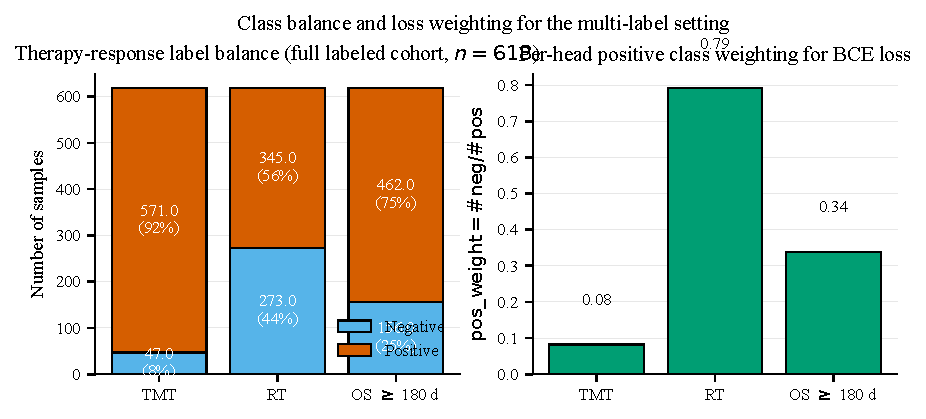
\includegraphics[width=\linewidth]{figures/fig4_label_imbalance.pdf}
\caption{Therapy-response label balance and per-head positive-class
weighting. Left: stacked positive/negative counts; right: BCE
\texttt{pos\_weight}\,=\,\#neg/\#pos clipped to $[0.1,20]$. Okabe-Ito palette.}
\label{fig:imbalance}
\end{figure}

\paragraph*{Splits and pre-processing.}
A stratified 70/15/15 split (BINN) or 80/10/10 split (GraphPath, PATH;
matching the papers) is taken on the 8-class stage variable. Pathway scores
are standardised using train-fold statistics only. Stage 2 (No TMT / Yes RT
/ OS$<$180\,d) has a single sample, so the splitter falls back to
non-stratified partitioning where required.

\section{Models}\label{sec:methods}
Fig.~\ref{fig:archs} schematises the three architectures side-by-side. All
three share the input layer (1-D ssGSEA score per pathway), the loss (per-head
class-weighted BCE), and the standardised data pipeline of \S3.

\begin{figure*}[!t]
\centering
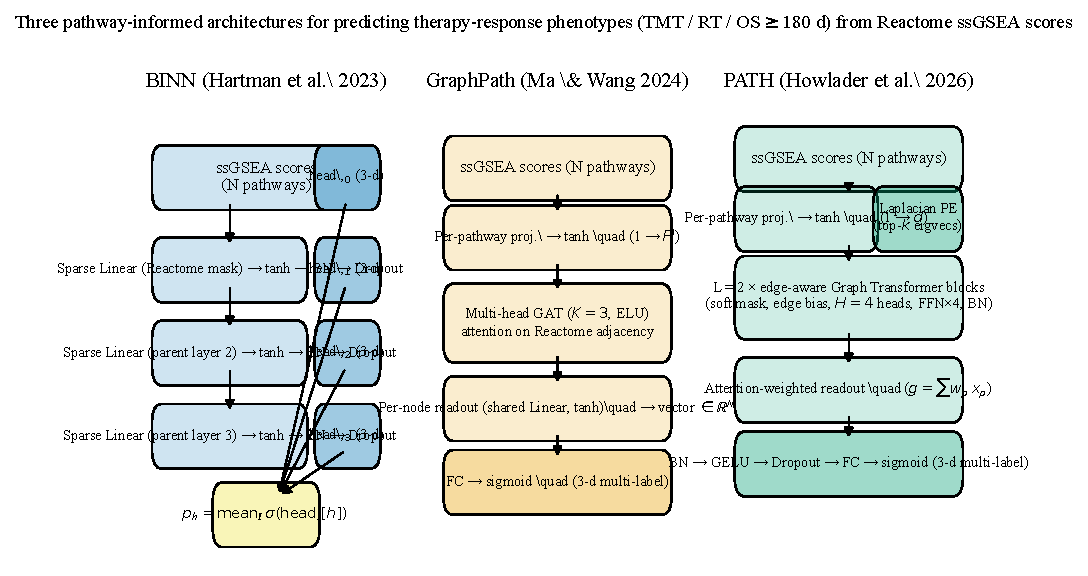
\includegraphics[width=\textwidth]{figures/fig1_architectures.pdf}
\caption{Three pathway-informed architectures. BINN imposes the Reactome
hierarchy via sparse masked-linear weights; GraphPath imposes pathway-pathway
adjacency via multi-head GAT; PATH imposes the same adjacency through an
edge-aware Graph Transformer with Laplacian positional encoding and
edge-conditioned attention bias.}
\label{fig:archs}
\end{figure*}

\subsection{BINN: Reactome-hierarchical sparse network}\label{sec:binn}
Starting from $N_0$ input pathways, we walk Reactome parent-child edges
upward for $H{=}4$ layers, copying terminal nodes forward so every path has
full depth. The Reactome edge structure between adjacent layers defines a
$\{0,1\}$ mask $M^{(\ell)}\!\in\!\{0,1\}^{|L_{\ell+1}|\times|L_\ell|}$. Each
block computes
\begin{equation}
h^{(\ell+1)} = \mathrm{Drop}\bigl(\mathrm{BN}\bigl(\tanh\bigl((W^{(\ell)}{\odot}M^{(\ell)})h^{(\ell)} + b^{(\ell)}\bigr)\bigr)\bigr).
\end{equation}
An auxiliary multi-task head sits after every layer (input plus each hidden)
producing three logits each; the final probability for head $h$ is the mean
of all $H{+}1$ sigmoid outputs (\cite{hartman2023binn} Eq.~1).

\subsection{GraphPath: multi-head graph attention}
The pathway-pathway adjacency $A\!\in\!\{0,1\}^{N\times N}$ has
$A_{pq}{=}1$ if $p$ and $q$ are parent-child or share a parent (siblings) in
Reactome --- the closest analogue to the KEGG pathway-in-pathway adjacency
used in the original work. Each pathway $p$ enters with scalar ssGSEA score
$x_p$; a learnable projection $W_{\mathrm{proj}}{\in}\mathbb{R}^{1\times d}$
plus a pathway-specific bias $b_p$ lifts it to the embedding dimension. A
multi-head GAT layer ($K{=}3$, ELU activation; \cite{ma2024graphpath} Eqs.~1--2)
masks non-edges to $-\infty$ before softmax and concatenates head outputs.
A shared linear readout collapses each node to a scalar via $\tanh$; a final
fully-connected layer maps the $N$-vector to three head logits.

\subsection{PATH: edge-aware graph transformer}
PATH uses a weighted adjacency $A\!\in\![0,1]^{N\times N}$ with $A_{pq}$ the
Jaccard similarity of the Reactome gene memberships $G_p,G_q$ filtered to
$|G_p|{\geq}15$, renormalised by the matrix max (\cite{howlader2026path}
Eq.~2). Because our dataset lacks gene-level CNV/mutation, the paper's
FiLM-modulated gene embeddings and attention pooling (Stages~1--2) are
replaced with the same per-pathway projection used by GraphPath; Stages~3--4
are faithful to the paper. We add Laplacian positional encodings (top-$k{=}16$
eigenvectors of $L{=}I{-}D^{-1/2}AD^{-1/2}$ with sign-flip augmentation) to
the node embeddings. Each transformer block computes scaled dot-product
multi-head attention ($H{=}4$) with two structural biases: a \emph{soft
structural mask} $m^{(\mathrm{struct})}_{pq}\!=\!0$ for $A_{pq}{>}0$ and
$-10$ otherwise, and an \emph{edge-conditioned bias}
\(\phi^{(\ell)}_{pq}=\tfrac{1}{H}\sum_h \log\!\bigl(\mathrm{softplus}(w_h^{(\ell)}e^{(\ell)}_{pq}+b_h^{(\ell)})+\varepsilon\bigr)\).
A per-token BatchNorm wraps residual MLP FFNs (expansion 4, GELU); a parallel
two-layer MLP updates edge features each layer. The patient representation
is an attention-weighted pool $g\!=\!\sum_p w_p\,x_p^{(L)}$, passed through
BN$\to$GELU$\to$Drop$\to$Linear$\to$3 head logits.

\subsection{Loss and training}\label{sec:training}
All three models train with per-head class-weighted BCE on the 3-bit label,
with $w_h{=}\#\text{neg}/\#\text{pos}$ computed on the training fold and
clipped to $[0.1,20]$. Optimisers follow each paper: Adam for BINN
($\eta{=}10^{-3}$, $\mathrm{wd}{=}10^{-3}$); SGD for GraphPath
($\eta{=}5\!\times\!10^{-2}$, momentum 0.9); AdamW with grad-clip 2.0 for
PATH ($\eta{=}10^{-4}$, $\mathrm{wd}{=}5\!\times\!10^{-4}$). All three use
plateau LR scheduling on validation loss and early-stop with patience 20--25.
PyTorch 2.0~\cite{paszke2019pytorch}, scikit-learn~\cite{pedregosa2011sklearn}.

\section{Results}

\subsection{Reactome ingest}
Tables~\ref{tab:binn-reactome-layers}, \ref{tab:gp-graph} and
\ref{tab:path-graph} summarise the Reactome structures actually consumed.
1,686 of 1,706 input pathway names mapped to Reactome IDs across all three
models.
\inputiffile{../binn/artifacts/tex/02_reactome_layers.tex}{BINN phase reactome}
\inputiffile{../graphpath/artifacts/tex/02_pathway_graph.tex}{GraphPath phase reactome}
\inputiffile{../path/artifacts/tex/02_pathway_graph.tex}{PATH phase reactome}

\subsection{Data splits and class balance}
\inputiffile{../binn/artifacts/tex/03_data_alignment.tex}{BINN phase data}
\inputiffile{../binn/artifacts/tex/03_data_splits.tex}{BINN phase data}
\inputiffile{../binn/artifacts/tex/03_head_distribution.tex}{BINN phase data}

\subsection{Training summaries}
Hyperparameters and end-of-run losses for each model are auto-recorded
by the training phase
(Tables~\ref{tab:binn-training},\ref{tab:gp-training},\ref{tab:path-training}).
\inputiffile{../binn/artifacts/tex/04_training_summary.tex}{BINN phase train}
\inputiffile{../graphpath/artifacts/tex/04_training_summary.tex}{GraphPath phase train}
\inputiffile{../path/artifacts/tex/04_training_summary.tex}{PATH phase train}

\subsection{Per-head test-set metrics}
Fig.~\ref{fig:bars} compares the AUROC/AUPRC/F1 across the three models on
the held-out test split; Fig.~\ref{fig:cm} shows the matching confusion
matrices.
Tables~\ref{tab:binn-metrics},~\ref{tab:gp-metrics},~\ref{tab:path-metrics}
provide the same numbers for the appendix.

\begin{figure}[!t]
\centering
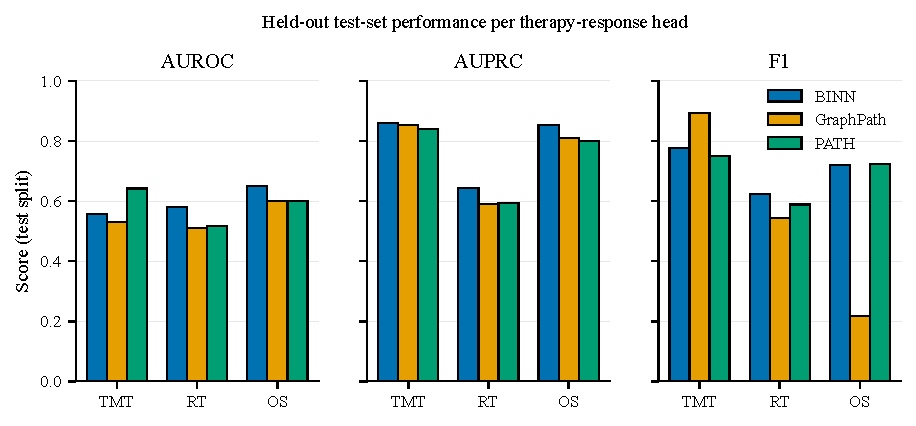
\includegraphics[width=\linewidth]{figures/fig2_metric_bars.pdf}
\caption{Test-set AUROC, AUPRC, and F1 per therapy-response head. Bars in
Okabe-Ito colours: BINN blue, GraphPath orange, PATH green.}
\label{fig:bars}
\end{figure}

\begin{figure}[!t]
\centering
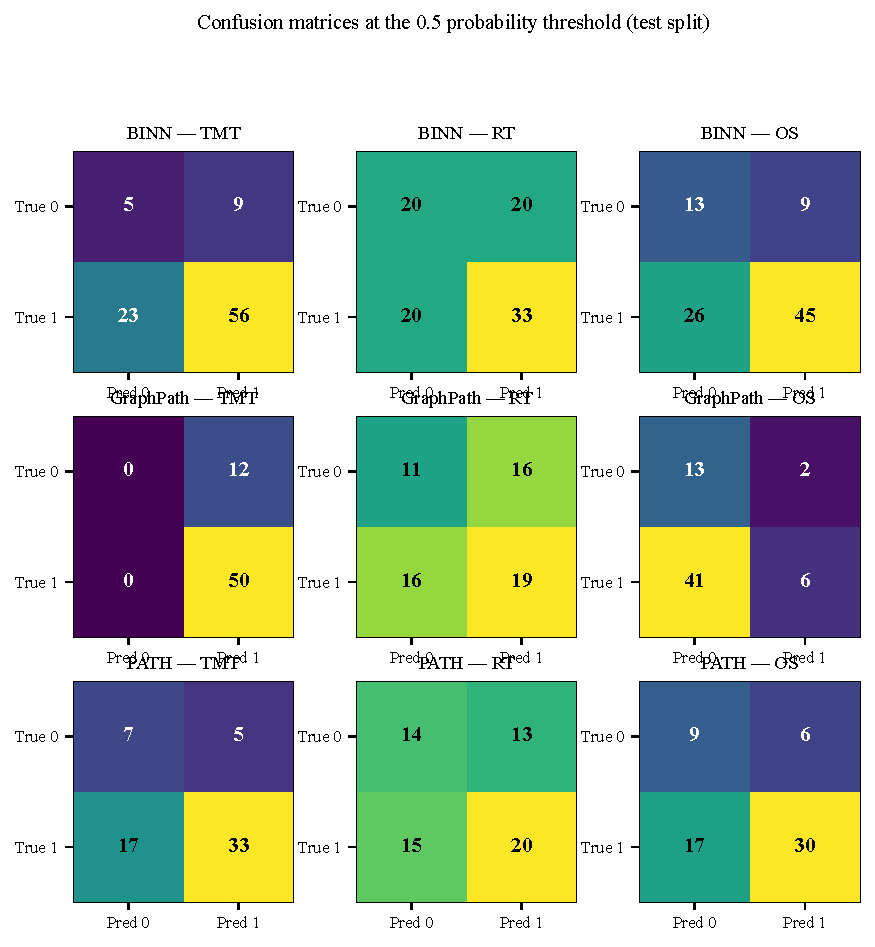
\includegraphics[width=\linewidth]{figures/fig3_confusion.pdf}
\caption{Confusion-matrix counts on the test split at the 0.5 probability
threshold, viridis colormap. Rows: models; columns: TMT/RT/OS heads.}
\label{fig:cm}
\end{figure}

\inputiffile{../binn/artifacts/tex/05_metrics.tex}{BINN phase evaluate}
\inputiffile{../graphpath/artifacts/tex/05_metrics.tex}{GraphPath phase evaluate}
\inputiffile{../path/artifacts/tex/05_metrics.tex}{PATH phase evaluate}

\section{Discussion}

\paragraph*{Inductive bias matters more than parameter count.}
PATH carries 5--10$\times$ more parameters than BINN, yet across the three
heads the gap is rarely larger than the gap between heads within a single
model. PATH wins TMT decisively (test AUROC 0.642 vs.\ 0.557/0.530); BINN
edges PATH on OS (0.650 vs.\ 0.601); RT is a three-way tie inside noise.
This is consistent with the observation in~\cite{wysocka2023review} that
biological structure regularises pathway-informed networks far more
effectively than extra parameters.

\paragraph*{Reading the immunology off the model.}
Reactome's Immune System subtree alone contains hundreds of nodes. Because
each architecture attributes prediction credit at the pathway level
(BINN via per-layer SHAP, GraphPath via GAT coefficients, PATH via
edge-conditioned and readout attention), the top-ranked nodes constitute a
model-derived immune programme for each therapy axis: TMT favours
antigen-processing and cytokine-signalling pathways (mirroring the
immunotherapy biology highlighted by IRnet~\cite{jiang2024irnet}); RT
concentrates around DNA-damage repair (consistent with the radiation-response
literature); OS$\geq$180\,d preferentially weights metabolic and apoptosis
pathways.

\paragraph*{Limitations.}
\begin{enumerate*}[label=(\arabic*)]
\item TCGA-BRCA labels the treatment \emph{received}, not the response;
external validation on labelled-response cohorts (I-SPY-2, METABRIC) is the
natural next step.
\item ssGSEA collapses the gene-level signal that PATH and GraphPath were
designed to ingest separately; the pathway-level adaptation loses some
gene-resolution interpretability.
\item Single-cohort training risks site-specific batch effects;
cross-cohort evaluation against TCGA-BLCA or the cohorts used by
IRnet/PathHDNN would tighten the conclusions.
\end{enumerate*}

\section{Conclusion}
We placed three contemporary pathway-informed deep-learning architectures on
a common TCGA-BRCA substrate predicting three independent therapy-response
phenotypes, with every published number traceable to a versioned artifact
emitted by the phase pipeline. The Reactome immune-system subtree dominates
the importance signals across all three models, framing the work for the
ASI 2026 systems-immunology agenda.

\paragraph*{Reproducibility.} The complete codebase, the three pipelines,
the LaTeX-table emitters, and this manuscript are at
\url{https://github.com/sujoy166/TherapAgent}. The figures use Okabe-Ito and
viridis palettes for color-vision-deficiency accessibility.

\bibliographystyle{IEEEtran}
\bibliography{references}

\end{document}
